\documentclass{article}
\usepackage{amsmath}
\usepackage{amssymb}
\usepackage[pdftex]{graphicx}
\usepackage[]{mcode}
\usepackage{pgfplots}

\pdfpagewidth 8.5in
\pdfpageheight 11in
\topmargin -1in
\headheight 0in
\headsep 0in
\textheight 8.5in
\textwidth 6.5in
\oddsidemargin 0in
\evensidemargin 0in 
\headheight 50pt
\headsep 0in
\footskip .75in

\title{STA 601 - Lab 2}
\author{Kedar Prabhudesai}
\date{September 12, 2013}

\begin{document}
\maketitle

\begin{enumerate}
\item \underline{Normal-Gamma Model:}\\

$X|\tau^2 \sim Normal(0,1/\tau^2)$ and $\tau^2 \sim Gamma(\nu/2,\nu/2).$ To find the Marginal Distribution, $p(X)$

\begin{align*}
p(X) &= \int_{0}^{\infty} p(X|\tau^2)p(\tau^2)d\tau^2\\
		 &= \int_{0}^{\infty} \frac{\tau}{\sqrt{2\pi}} exp\left(\frac{-x^2\tau^2}{2}\right) \frac{(\nu/2)^{(\nu/2)}}{\Gamma(\nu/2)} (\tau^2)^{(\nu/2-1)} exp\left(\frac{-\nu\tau^2}{2}\right)d\tau^2\\
		 &= \frac{(\nu/2)^{(\nu/2)}}{\sqrt{2\pi}\Gamma(\nu/2)} \int_{0}^{\infty} \left(\tau^2\right)^{\frac{\nu+1}{2}-1} exp\left[-\tau^2\left(\frac{x^2+\nu}{2}\right)\right] d\tau^2\\
		 &= \frac{(\nu/2)^{(\nu/2)}}{\sqrt{2\pi}\Gamma(\nu/2)} \frac{\Gamma(\frac{\nu+1}{2})}{\left( \frac{x^2+\nu}{2}\right)^{\frac{\nu+1}{2}}} \int_{0}^{\infty} \frac{\left( \frac{x^2+\nu}{2}\right)^{\frac{\nu+1}{2}}}{\Gamma(\frac{\nu+1}{2})} \left(\tau^2\right)^{\frac{\nu+1}{2}-1} exp\left[-\tau^2\left(\frac{x^2+\nu}{2}\right)\right] d\tau^2\\
		 &= \frac{(\nu/2)^{(\nu/2)}\Gamma(\frac{\nu+1}{2})}{\sqrt{2\pi}\Gamma(\nu/2)} \left( \frac{x^2+\nu}{2}\right)^{-\frac{\nu+1}{2}}\\ 
p(X) &\propto \left( \frac{x^2+\nu}{2}\right)^{-\frac{\nu+1}{2}}\\
p(X) &\propto \left( \frac{x^2/\nu+1}{2/\nu}\right)^{-\frac{\nu+1}{2}}\\
p(X) &\propto \left[ \left(1+\frac{x^2}{\nu}\right) \left(\frac{\nu}{2}\right)\right]^{-\frac{\nu+1}{2}}\\
p(X) &\propto \left(1+\frac{x^2}{\nu}\right)^{-\frac{\nu+1}{2}}\\
\end{align*}
\noindent Therefore, we can say that $X\sim$ T-Distribution with $\nu$ Degrees of Freedom.

\pagebreak
\item Given is histogram of samples from $X|\tau^2.$ The samples do look like they are drawn from a T-Distribution with $\nu=1.$ Because, it was a heavy tailed distribution, I did have extreme values. I have provided here a zoomed plot of the histogram. T-Distribution with $\nu=1$ is also called 'The Cauchy Distribution'.\\

\begin{center}
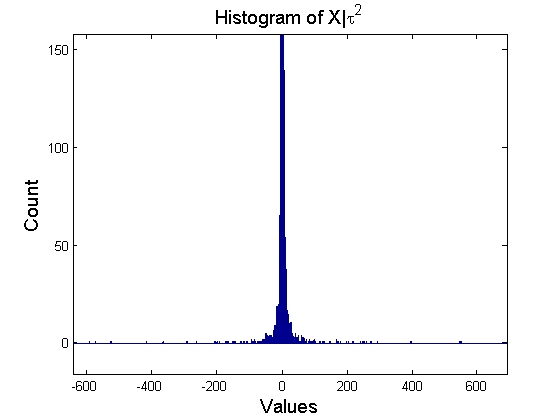
\includegraphics[scale=0.5]{XGivenT2Hist.png}\\
\end{center}

\item Running KS-Test in Matlab I got, $p=0.7528.$

\item This is a histogram of $1000$ p-values. For me it looks more or less (but not quite) like a normal. I know it is supposed to look like a Uniform which would be $Beta(1,1).$ But looking at this one I don't think I can say that. Not sure why it looks like this. 

\begin{center}
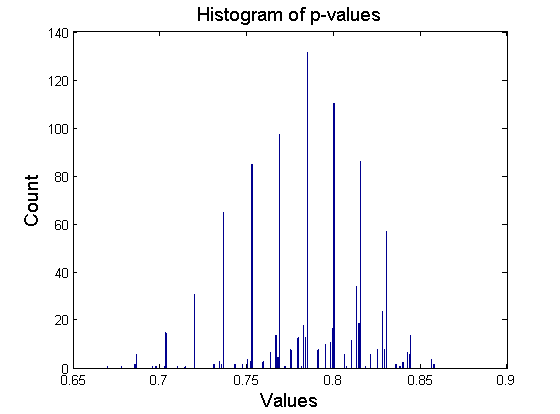
\includegraphics[scale=0.5]{pValHist.png}\\
\end{center}

\item The Central Limit Theorem (CLT) states that, the arithmetic mean of a sufficiently large number of independent samples of a random variable, will be approximately normally distributed. \\

For $\nu=1$, the Mean and Variance of the t-distribution is 'Not Defined'. Hence the CLT will not hold.\\

For $\nu=2$, the mean is 0, but the variance is $\infty.$ ('Infinity' which is different from 'Not Defined'). This also imples that because of large variance in our samples, we will not converge to a normal distribution.\\

For $\nu=3$, the mean is 0 and variance is $\frac{\nu}{\nu-2}$. In this case we can say that we will converge to a normal distribution if we draw a large number of samples from the t-distribution.\\

\end{enumerate}
\end{document}